

\documentclass[12pt]{article}

\usepackage{blindtext} % Package to generate dummy text throughout this template 
\usepackage{graphicx}
\usepackage{float}
\graphicspath{./ } 
\usepackage[sc]{mathpazo} % Use the Palatino font
\usepackage[T1]{fontenc} % Use 8-bit encoding that has 256 glyphs
\linespread{1.5} % Line spacing - Palatino needs more space between lines
\usepackage{microtype} % Slightly tweak font spacing for aesthetics

\usepackage[english]{babel} % Language hyphenation and typographical rules

\usepackage[hmarginratio=1:1,top=32mm,columnsep=20pt]{geometry} % Document margins
\usepackage[hang, small,labelfont=bf,up,textfont=it,up]{caption} % Custom captions under/above floats in tables or figures
\usepackage{booktabs} % Horizontal rules in tables

\usepackage{lettrine} % The lettrine is the first enlarged letter at the beginning of the text

\usepackage{enumitem} % Customized lists
\setlist[itemize]{noitemsep} % Make itemize lists more compact

\usepackage{abstract} % Allows abstract customization
\renewcommand{\abstractnamefont}{\normalfont\bfseries} % Set the "Abstract" text to bold
\renewcommand{\abstracttextfont}{\normalfont\small\itshape} % Set the abstract itself to small italic text

\usepackage{titlesec} % Allows customization of titles
\renewcommand\thesection{\Roman{section}} % Roman numerals for the sections
\renewcommand\thesubsection{\roman{subsection}} % roman numerals for subsections
\titleformat{\section}[block]{\large\scshape\centering}{\thesection.}{1em}{} % Change the look of the section titles
\titleformat{\subsection}[block]{\large}{\thesubsection.}{1em}{} % Change the look of the section titles

\usepackage{fancyhdr} % Headers and footers
\pagestyle{fancy} % All pages have headers and footers
\fancyhead{} % Blank out the default header
\fancyfoot{} % Blank out the default footer
\fancyfoot[RO,LE]{\thepage} % Custom footer text

\usepackage{titling} % Customizing the title section

\usepackage{hyperref} % For hyperlinks in the PDF

%----------------------------------------------------------------------------------------
%	TITLE SECTION
%----------------------------------------------------------------------------------------

\setlength{\droptitle}{-4\baselineskip} % Move the title up

\pretitle{\begin{center}\Huge\bfseries} % Article title formatting
	\posttitle{\end{center}} % Article title closing formatting
\title{Finding Similar Items} % Article title

\author{%
	\textsc{Sainey Manga - ID 943874}\\[1ex] % Your name
	\normalsize University of Milan, Data Science and Economics \\ % Your institution
	\normalsize \href{mailto:sainey.manga@studenti.unimi.it}{sainey.manga@studenti.unimi.it} % Your email address
	%\and % Uncomment if 2 authors are required, duplicate these 4 lines if more
	%\textsc{Jane Smith}\thanks{Corresponding author} \\[1ex] % Second author's name
	%\normalsize University of Utah \\ % Second author's institution
	%\normalsize \href{mailto:jane@smith.com}{jane@smith.com} % Second author's email address
}
\date{\today} % Leave empty to omit a date
\renewcommand{\maketitlehookd}{%

}

%----------------------------------------------------------------------------------------

\begin{document}
	
	% Print the title
	\maketitle
	
	%----------------------------------------------------------------------------------------
	%	ARTICLE CONTENTS
	%----------------------------------------------------------------------------------------
	
	I/We declare that this material, which I/We now submit for assessment, is entirely my/our own work and has not been taken from the work of others, save and to the extent that such work has been cited and acknowledged within the text of my/our work. I/We understand that plagiarism, collusion, and copying are grave and serious offences in the university and accept the penalties that would be imposed should I engage in plagiarism, collusion or copying. This assignment, or any part of it, has not been previously submitted by me/us or any other person for assessment on this or any other course of study.
	\section{Introduction}
	
	\lettrine[nindent=0em,lines=3]{W} ith advances in data collection techniques and extended storage media volume of stored data is growing constantly. As an example, all pages stored in internet can be noted. With the increasing volume of data stored, it is not possible retrieving them with conventional techniques easily. Therefore, methods for processing massive data are required. A fundamental data-mining problem is to examine data for “similar” items. The problem of finding textually similar documents is one of the problems of finding similar items. 
\\
	The aim of this project is to implement a detector of pairs of similar items, analyzing the stack sample dataset published on Kaggle. The project explores Local sensitive hashing approach design for Jaccard distance.

	
	%------------------------------------------------
	
	\section{DATA DESCRIPTION AND PREPROCESSING}
	
	The data set \href{https://www.kaggle.com/stackoverflow/stacksample}{stacksample}   downloaded from Kaggle where it is published and released under the CC-BY-SA 3.0 license. It is downloaded during code execution via the Kaggle API. The entire data set consists of three different tables, namely:
	\begin{itemize}
		\item Questions which contains the title, body, creation date, closed date (if applicable), score, and owner ID for all non-deleted Stack Overflow questions whose Id is a multiple of 10.
		\item Answers which contains the body, creation date, score, and owner ID for each of the answers to these questions. The Parent-Id column links back to the Questions table.
		\item Tags which contains the tags on each of these questions.
	\end{itemize}

	In this this project, we are only interested on only the table “Questions” where we considered the attribute “body” as the set of documents or items we will mined for similarity. A function was implemented using spark to read and curate only the body and id of the required table, other attributes were filtered out from the table. 
\\
	After loading the data set, a function called \textbf{clean\_text()} was defined to remove all characters, html links, numbers and other unwanted features found on the text of the body attribute. 
\\
	The first 10 rows of cleaned data are shown below: \\
	\begin{figure}[H]
		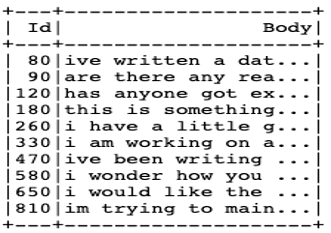
\includegraphics[scale=1]{dataset.png}
		\centering
		\caption{First ten rows of the data set}
		\label{fig:dataset}
	\end{figure}
	A tokenization process was caried on the cleaned data set to distinctly separate the text into pieces (tokens). This was done with the help of the RegexTokenizer function in pyspark.ml.feature.\\
	To remove the low-level information from our text, we also removed stop words from the corpus so that we can focus on the more important words in the text. We fed the tokens generated from the previous step onto the function StopWordsRemover in pyspark.ml.feature.
		\begin{figure}[H]
		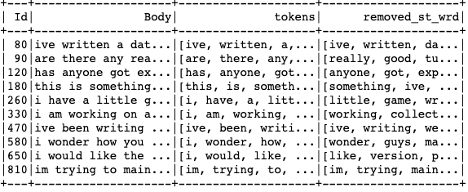
\includegraphics[scale=0.8]{tokenize.png}
		\centering
		\caption{Tokenized with removed stop words data}
		\label{fig:token}
	\end{figure}

	
	%------------------------------------------------
	
	\section{ALGORITHMS AND IMPLEMENTATION}
	\subsection{Jaccard Similarity}
	In this project, the Jaccard similarity algorithm was implemented to find the pair of questions that are similar in the data set. The Jaccard similarity and Jaccard distance are differentiated by the mathematical definition. The similarity is subtracted from one (1) to have the distance. If the similarity approach is to be considered, then more similar items have a score closer to one and a score closer to zero if otherwise.
\\
	The Jaccard similarity is defined as:
		\begin{equation}
		\label{eq:emc}
		SIM(A, B) = \frac{|A \cap B|}{|A \cup B|}
		\end{equation}
	\subsection{Local Sensitive Hashing (LSH) for Minhashing}
	One general approach to LSH is to “hash” items several times, in such a way that similar items are more likely to be hashed to the same bucket than dissimilar items are. This is applied in large data sets to reduce the computational costs, so that items that are more likely to be similar are considered.
	
	
	%------------------------------------------------
	
	\section{EXPERIMENTS AND RESULTS}
	The experiments carried out on this project are done through the help of spark. Firstly, a pipeline model was set to implement two very key functions. The function HashingTF from pyspark which maps a sequence of terms to their term frequencies using the hashing trick. It takes in as input the text where stop words have been removed and outputs a column of vectors to be used for hashing. Finally, the LSH class for Jaccard distance was also implemented in the pipeline model through the MinHashLSH function from pyspark.
\\
	The function takes in as input the sparse vector generated from the previous step and outputs the hashes which we shall use for the implementation of our Jaccard distance.
\\
			\begin{figure}[H]
		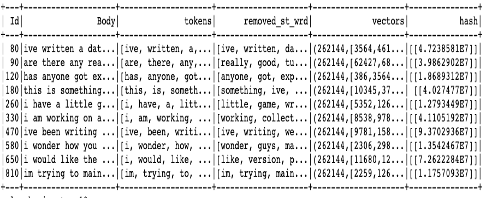
\includegraphics[scale=0.9]{hash.png}
		\centering
		\caption{Data showing the vectors and hashes}
		\label{fig:hash}
	\end{figure}
	To limit computational time, we implemented the final model on a sample of 40,000 from the data set. This is done after conducting the LSH minhashing. The approach is indeed scalable to large data sets. All rows were filtered out to take only the rows that have questions with at least a word.\\
	Finally, to implement the Jaccard distance model, the approxSimilarityJoin function in pyspark was invoked with a negative one [-1] to make it a distance. It takes as input the hashed data, where the data set has been divided into two parts with respect to the ids. The results are filtered to show only the pairs that have a similarity score below 0.7. This is to show only a reasonable number of pairs of similar items. \\
	\begin{figure}[H]
		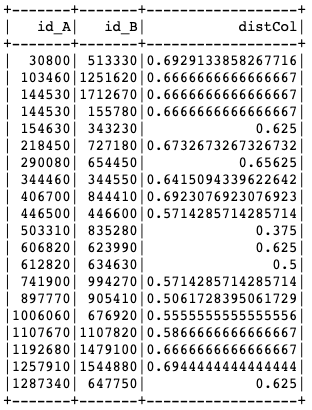
\includegraphics[scale=0.9]{similaritem.png}
		\centering
		\caption{Pairs of similar items}
		\label{fig:similaritem}
	\end{figure}
	The table \ref{fig:similaritem} shows two sets of ids representing to various texts with their corresponding similarity score. The closer the score is to zero, the more similar the texts are. We can see that the ids 503310 and 835280 are the most similar questions in the data set. This is followed by the score of 0.5.
\\
	We show below a sample of similar text as provided by the solution of the model implemented.
		\begin{figure}[H]
		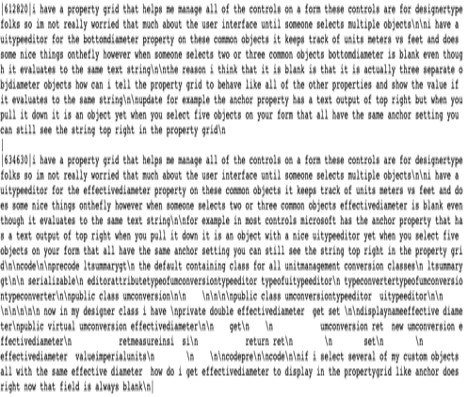
\includegraphics[scale=0.9]{sample.png}
		\centering
		\caption{IDs with score 0.5}
		\label{fig:sample}
	\end{figure}

\begin{figure}[H]
	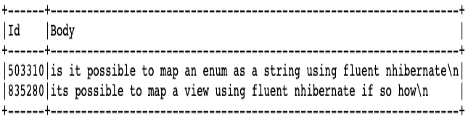
\includegraphics[scale=0.9]{sample2.png}
	\centering
	\caption{IDs with score 0.375}
	\label{fig:sample2}
\end{figure}
	\section{CONCLUSION}
	So far what we have seen in the two samples of results is that a pair could be classified similar, but the context of the two texts would be entirely different. For example, our most similar pair from the data set asked about two different things, but the questions have a similar format and a good number of similar words. With Jaccard distance, we know pairs with more common words would appear to be similar.
\\
	Summarily, the project utilized LSH class of Jaccard distance to find pairs of similar items from the StackSample data set. During model execution, the running time increased as we increased the size of the input data.
	
\end{document}
